%%%% FRACTIONAL OCTAVE SMOOTHING %%%%
\chapter{Log-symmetric fractional-octave smoothing}\label{chap:A3_Smoothing_Weights}
In this appendix, we reproduce a prior publication \citep{Tylka2017} in which we proposed a method for fractional-octave smoothing that, for spectra that are originally symmetric in log-frequency, preserves said symmetry after smoothing.
Unlike an existing method, which requires interpolation of the FFT spectra to a log-frequency scale, the proposed method uses analytically-derived smoothing windows and operates directly in the FFT domain, thereby retaining compatibility with well-established spectral smoothing techniques such as complex smoothing.
In this work, we compared the proposed method to two existing methods by smoothing the magnitude response of an analog band-pass filter (which is symmetric on a log-frequency scale) and subsequently calculating a ``center of mass'' of the smoothed spectra to quantify any loss of symmetry.
The first existing method uses symmetric (on a linear scale) smoothing windows, which exhibit the correct bandwidths but do not span the correct fractional-octave frequency ranges, whereas the second interpolates the spectrum to logarithmically-spaced frequencies and then uses a symmetric fixed-width smoothing window.
As reproduced below, the results of this study showed that the proposed method achieves nearly identical smoothed spectra to the second method, but without the need for interpolation, and that the first method indeed skews the log-symmetry of the original spectra.
Consequently, throughout the present thesis, we employ our proposed method for fractional-octave smoothing where needed (see, in particular, \secref{sec:04_Auditory_Models:Coloration_Metrics:Epk}).

\section{Introduction}\label{sec:A3_Smoothing_Weights:Introduction}
Frequency spectrum smoothing is a standard operation in many fields of audio and acoustics as it reduces the often overwhelming detail of high-resolution spectra to only the relevant information.
Perhaps its most common usage is to make frequency response data suitable for plotting.
However, smoothing is also useful when designing compensation filters for transducer equalization or room response correction, as it both reduces the dynamic range and creates a simplified model of the system to be equalized that, ideally, consists of only the perceptually-relevant information.
In such applications it is important that the peaks (and notches) of the compensation filter align with the corresponding notches (peaks) in the original response, since failure to cancel the notch (peak) may lead to an even worse overall response as a new peak (notch) will have been introduced.
Smoothing methods must therefore be employed carefully so that prominent features of the frequency response such as peaks and notches are not unintentionally shifted during the smoothing process.

One application of spectral smoothing is in the design of headphone equalization (EQ) filters, wherein the headphone transfer function (which describes the transmission of sound from the headphones to the listener's ear drums) is first smoothed and then either inverted and used directly as the EQ filter, or used to define a regularization function that improves the conditioning of the inversion operation and mitigates excessive boosting in the EQ filter \citep{ScharerLindau2009}.
Spectral smoothing is also used in binaural audio to reduce the complexity of the head-related transfer function (HRTF), which describes the transmission of sound from a point in space to a listener's ear drums.
As a listener's HRTF often contains more detailed spectral information than is perceptually relevant, measured HRTFs can be smoothed to a certain degree without loss of localization accuracy or externalization \citep{XieZhang2010, Hassager2014}.
This enables a simplified model of a listener's HRTF to be used to generate perceptually-accurate personalized binaural audio \citep{Rasumow2014}.

In these and other applications, it is often desired to obtain an impulse response after smoothing that retains the perceptually-relevant temporal features of the original impulse response.
To this end, \citet{HatziantoniouMourjopoulos2000} proposed ``complex smoothing,'' which extends the procedure of fractional-octave smoothing to complex-valued transfer functions (as opposed to the squared magnitude response used in traditional power-spectrum smoothing) and enables the calculation of a ``smoothed'' impulse response.
More recently, \citet{Volk2011} proposed a method that uses complex-valued smoothing windows (corresponding to exponentially-decaying time windows applied to the impulse response) to better approximate the temporal and spectral smoothing inherent to the human auditory system.
Also, as an alternative to complex smoothing, \citet{Bank2013} presented a method of modeling transfer functions by a finite number of parallel second-order filters (whose poles are typically logarithmically-spaced in frequency), and showed that this method achieves a frequency resolution similar to that of fractional-octave smoothing.
Due to this current interest in obtaining equivalent time-domain responses after smoothing, any new spectral smoothing method should either retain compatibility with complex smoothing or prescribe an alternative method of obtaining the smoothed impulse response.

% Review of previous work focusing on the remaining problems (questions or deficiencies) the present paper claims to contribute to solving
\subsection{Previous work and remaining problems}
Fractional-octave smoothing is a special case of spectral smoothing in which the bandwidth of the smoothing window is a constant percentage of the center frequency.
Consequently, to smooth frequency spectra obtained via the fast Fourier transform (FFT) of a discrete-time signal, wherein the spectral data points are uniformly spaced in frequency, the fractional-octave smoothing window must vary with frequency.
\citet{HatziantoniouMourjopoulos2000} presented a method and general framework for smoothing FFT-based frequency spectra to an arbitrary frequency resolution.
However, this method prescribes smoothing windows that are symmetric on a linear frequency scale (and therefore do not span the correct fractional-octave bands), which consequently introduces an error, as is shown in the present work.
\citet{Lipshitz1985} prescribe interpolating the FFT spectrum to a logarithmic frequency (log-frequency) scale, so that a fixed-width moving-average filter may be employed.
As is shown in the present work, this approach is able to preserve the log-symmetry of raw spectra but requires leaving the FFT domain via interpolation, incurring a computational cost and necessarily introducing errors.

% A statement of the paper's main question(s) and goal(s), followed by a succinct description of the general method and approach to be described in the paper
\subsection{Objectives and approach}
The goal of this work is to derive a fractional-octave smoothing method that preserves the log-symmetry of the original spectrum.
Ideally, such a method should also operate directly on FFT-based frequency spectra, without the need to interpolate to a non-uniform frequency scale, and should be compatible with complex smoothing.
Additionally, we evaluate the ability of existing fractional-octave smoothing methods to preserve log-frequency symmetry seen in the original spectrum.
To evaluate the methods considered in this work, we apply each method to the magnitude response of an analog band-pass filter, which is symmetric on a log-frequency scale.
Any loss of symmetry is examined in terms of a ``center of mass'' of the smoothed spectrum.

% A brief section by section description of the structure of the paper
In \secref{sec:A3_Smoothing_Weights:Smoothing_Methods} we present the framework for fractional-octave smoothing, followed by a brief review of the symmetric-window method in \secref{sec:A3_Smoothing_Weights:Smoothing_Methods:Hatziantoniou_Method} and the log-frequency interpolation method in \secref{sec:A3_Smoothing_Weights:Smoothing_Methods:Lipshitz_Method}.
We then propose an alternative method in \secref{sec:A3_Smoothing_Weights:Smoothing_Methods:Proposed_Method}, perform a comparative analysis of the three methods in \secref{sec:A3_Smoothing_Weights:Analysis}, and conclude.

\section{Smoothing methods}\label{sec:A3_Smoothing_Weights:Smoothing_Methods}
In general, spectral smoothing may be applied to any function of frequency.
Here, we restrict our discussion to raw (i.e., not smoothed) frequency spectra whose data points are specified at uniformly-spaced frequencies on a linear scale, such as those obtained through an FFT.
Furthermore, in the applications of spectral smoothing mentioned in the introduction, the spectra to be smoothed are typically frequency or magnitude responses of acoustic transfer functions, rather than Fourier transforms or power spectra of time-domain signals.\footnote{This distinction becomes necessary when discussing interpolation to a log-frequency scale.
For example, for power spectra of time-domain signals, conversion from a linear frequency scale to a log-frequency scale should also involve a change of units of the vertical axis, such that the values that are plotted on a linear frequency scale represent power per unit linear frequency, whereas those plotted on a log-frequency scale represent power per unit log-frequency.
Through this conversion, a pink-noise power spectrum plotted over linear frequency would exhibit the usual $-3$~dB/octave slope, while on a log-scale, the spectrum would appear flat.
Consequently, on either frequency scale, integrating the power spectrum over a given frequency band gives the total power in that band.
However, for frequency (or magnitude) responses of transfer functions, the values that are plotted are gains for specific frequencies, regardless of the distribution of those frequency points.
Consequently, interpolation of a frequency response to a log-frequency scale should involve only a ``resampling'' of the response to logarithmically-spaced frequencies; it should not involve a change of units.} Consequently, we further restrict our discussion to the smoothing of frequency or magnitude responses of transfer functions.

Consider a raw, possibly complex-valued frequency spectrum of length $N$ denoted by $X[k]$, where $k$ is the discrete frequency index.
The smoothed spectrum is given by
\begin{equation}\label{eq:A3_Smoothing_Weights:SmoothingSummation}
X_\textrm{s}[k] = \sum_{k' = 0}^{N - 1} W[k, k'] X[k']
\end{equation}
for all integers $k,k' \in [0, N - 1]$, where, for a given value of $k$, $W[k, k']$ denotes the $k^{\textrm{th}}$ sequence of non-negative weights used to smooth the raw spectrum \citep{HatziantoniouMourjopoulos2000}.
These weights are normalized such that, for all $k \in [0, N - 1]$,
\begin{equation}\label{eq:A3_Smoothing_Weights:WeightNorm}
\sum_{k' = 0}^{N - 1} W[k, k'] = 1.
\end{equation}

The smoothing operation defined by \eqnref{eq:A3_Smoothing_Weights:SmoothingSummation} can be thought of as a frequency-domain convolution with a frequency-dependent kernel, $W[k, k']$.
In the case of a frequency-invariant smoothing window (e.g., a fixed-width moving-average filter), we can instead define a single weight sequence $W[k - k'] = W[k, k']$, and \eqnref{eq:A3_Smoothing_Weights:SmoothingSummation} takes the standard form of convolution.

To compute the smoothed spectrum at a given frequency $f = k F_s / N$, where $F_s$ is the sampling rate, the (exact) lower and upper cutoff frequencies of the weighting function are given by
\begin{equation}\label{eq:A3_Smoothing_Weights:cutoffs}
    \begin{array}{ll}
    f_L &= f \cdot 2^{-\Delta/2},\\[8pt]
    f_U &= f \cdot 2^{+\Delta/2},
    \end{array}
\end{equation}
respectively \citep{HatziantoniouMourjopoulos2000}, where $\Delta$ is the smoothing bandwidth in octaves.
Consequently, the ratio, $Q$, of the center frequency to the bandwidth is a constant, and its reciprocal is given by
\begin{equation}\label{eq:A3_Smoothing_Weights:QFactor}
\frac{1}{Q} = \frac{f_U-f_L}{f} = 2 \sinh \left( \frac{\Delta \log (2)}{2} \right).
\end{equation}

%%%% Hatziantoniou's Method %%%%
\subsection{Method 1: symmetric weights} \label{sec:A3_Smoothing_Weights:Smoothing_Methods:Hatziantoniou_Method}
In the method presented by~\citet{HatziantoniouMourjopoulos2000}, the smoothed spectrum is computed using~\eqnref{eq:A3_Smoothing_Weights:SmoothingSummation}, where the weighting function is derived by first defining the half-length of the $k^{\textrm{th}}$ weight sequence as
\begin{equation}\label{eq:A3_Smoothing_Weights:HatzHalfWidth}
m[k] = \left\lfloor \frac{1}{2}\frac{k}{Q} \right\rfloor,
\end{equation}
where $\lfloor \cdot \rfloor$ denotes rounding down to the nearest integer.
The weighting function for a rectangular window is then given by
\begin{equation}\label{eq:A3_Smoothing_Weights:HatzWeights}
W_{\textrm{R}}[k, k'] = \left\{
    \begin{array}{cl}
	\displaystyle \frac{1}{2 m[k] + 1} & \textrm{for } \left| k - k' \right| \leq m[k],\\[8pt]
	0 & \textrm{for } \left| k - k' \right| > m[k].
    \end{array}\right.
\end{equation}
From this definition we see that each weight sequence is a rectangular window with $2 m[k] + 1$ non-zero values centered around $k = k'$.
This is in conflict with~\eqnref{eq:A3_Smoothing_Weights:cutoffs}, as the upper cutoff frequency should be further from the center than the lower cutoff, but instead the two ends of the weight sequence are equidistant to the center.
As we will show in~\secref{sec:A3_Smoothing_Weights:Analysis}, this error becomes significant for large smoothing bandwidths.

%%%% Lipshitz' Method %%%%
\subsection{Method 2: interpolation to logarithmic scale} \label{sec:A3_Smoothing_Weights:Smoothing_Methods:Lipshitz_Method}
In the method proposed by~\citet{Lipshitz1985}, the raw spectrum is first interpolated to a logarithmic frequency scale, at which point a fixed-width moving-average filter is applied.
The authors suggest interpolating to $N/2$ logarithmically-spaced frequencies, which we denote $\kappa[\ell]$, given by
\begin{equation}
\kappa[\ell] = \left( \frac{N}{2} \right)^\frac{\ell}{N/2-1},
\end{equation}
such that $1 \leq \kappa[\ell] \leq N/2$ for all integers $\ell \in [0, N/2 - 1]$.
The interval in octaves between any two adjacent frequencies is a constant, given by
\begin{equation}
\beta = \log_2 \frac{\kappa[\ell + 1]}{\kappa[\ell]} = \frac{1}{N/2-1} \log_2 \frac{N}{2},
\end{equation}
and, as we did for method 1, we define the weight-sequence half-length, $\mu$, as
\begin{equation}
\mu = \left\lfloor \frac{\Delta/2}{\beta} \right\rfloor,
\end{equation}
which is also constant.

To perform the interpolation,~\citet{Lipshitz1985} suggest a 4-point polynomial (i.e., cubic) interpolation, but, in general, any interpolation scheme (e.g., linear, spline, etc.) may be employed.
Here, we use linear interpolation, such that the interpolated raw spectrum, $\hat{X}$, which is now a function of the log-frequency index $\ell$, is given by
\begin{equation}\label{eq:A3_Smoothing_Weights:LogInterpolate}
\hat{X}[\ell] = X[k_1] + \left( X[k_2] - X[k_1] \right) \frac{\kappa[\ell] - k_1}{k_2 - k_1},
\end{equation}
where $k_1 = \big\lfloor \kappa[\ell] \big\rfloor$ and $k_2 = k_1 + 1$.

The smoothed spectrum, $\hat{X_\textrm{s}}$, is also a function of $\ell$ and is given by
\begin{equation}
\hat{X_\textrm{s}}[\ell] = \sum_{\ell' = 0}^{N/2 - 1} \hat{W}[\ell - \ell'] \hat{X}[\ell'],
\end{equation}
where $\hat{W}$ is the weighting function.
For a rectangular window, $\hat{W}$ is given by
\begin{equation}
\hat{W}_{\textrm{R}}[\ell - \ell'] = \left\{
    \begin{array}{cl}
	\displaystyle \frac{1}{2 \mu + 1} & \textrm{for } \left| \ell - \ell' \right| \leq \mu,\\[8pt]
	0 & \textrm{for } \left| \ell - \ell' \right| > \mu.
    \end{array}\right.
\end{equation}
The smoothed spectrum is then interpolated back to a linear frequency scale by
\begin{equation}
X_\textrm{s}[k] = \hat{X_\textrm{s}}[\ell_1] + \left( \hat{X_\textrm{s}}[\ell_2] - \hat{X_\textrm{s}}[\ell_1] \right) \frac{k - \kappa[\ell_1]}{\kappa[\ell_2] - \kappa[\ell_1]},
\end{equation}
where $\ell_1 = \left\lfloor (N/2 - 1) \log_{N/2} (k) \right\rfloor$ and $\ell_2 = \ell_1 + 1$.

%%%% Proposed Method %%%%
\subsection{Method 3: logarithmically-compensated weights} \label{sec:A3_Smoothing_Weights:Smoothing_Methods:Proposed_Method}
Consider a window $w(\phi)$ that is a function of the continuous variable $\phi$ (we will see later that $\phi$ is related to frequency).
Let $w$ be an even function of $\phi$ whose total integral is unity, i.e.,
\begin{equation}\label{eq:A3_Smoothing_Weights:WindowNorm}
\int_{-\infty}^{\infty} w(\phi) d\phi = 1.
\end{equation}

For example, given a smoothing bandwidth of $\Delta$ octaves, the normalized rectangular window is given by
\begin{equation}\label{eq:A3_Smoothing_Weights:RectangularWindowLogf}
w_\textrm{R}(\phi) = \left\{
    \begin{array}{cl}
	1/\Delta & \textrm{for } |\phi| \leq \Delta/2,\\[8pt]
	0 & \textrm{for } |\phi| > \Delta/2.
    \end{array}\right.
\end{equation}

For a given center-frequency index, $k$, we compute the weighting function by successively integrating adjacent slices of the window function, i.e.,
\begin{equation}\label{eq:A3_Smoothing_Weights:WeightsIntegral}
W[k, k'] = \int_{\Phi[k, k' - 0.5]}^{\Phi[k, k' + 0.5]} w(\phi) d\phi
\end{equation}
for all integers $k,k' \in [0, N - 1]$, where $\phi$ represents log-frequency in octaves relative to $k$, i.e., $\log_2(k'/k)$, and the limits of integration are given by
\begin{equation}\label{eq:A3_Smoothing_Weights:WeightsIntegralLimits}
\Phi[k, k' \pm 0.5] = \log_2 \left( \frac{k' \pm 0.5}{k} \right).
\end{equation}
As for method 1, the smoothed spectrum is then computed using~\eqnref{eq:A3_Smoothing_Weights:SmoothingSummation} but with this new weighting function.
Due to the normalization of the window function imposed in~\eqnref{eq:A3_Smoothing_Weights:WindowNorm}, each resulting weight sequence is also normalized and satisfies~\eqnref{eq:A3_Smoothing_Weights:WeightNorm}.

%% Example %%
%\begin{example*}
\paragraph*{Example:} To illustrate the difference between the calculated weights and the window function, consider the weight sequence needed to compute the value of the smoothed spectrum at $k = 10$, for 1-octave smoothing.
The window function is given by \eqnref{eq:A3_Smoothing_Weights:RectangularWindowLogf}, and the weights will be non-zero for, at most, $\lfloor k \cdot 2^{-\Delta/2} \rfloor \leq k' \leq \lceil k \cdot 2^{+\Delta/2} \rceil$, i.e., $k' \in [7, 15]$, where $\lceil \cdot \rceil$ denotes rounding up to the nearest integer and the bounds of the inequalities are obtained by substituting $k$ for $f$ in~\eqnref{eq:A3_Smoothing_Weights:cutoffs}.
However, integrating the window function for all slices reveals that $W[10,15] = 0$, since that integral begins at $\log_2 (14.5/10)$ but the window function already dropped to zero at $\phi \approx \log_2 (14.142/10)$.

\begin{figure}[t]
    \centering
    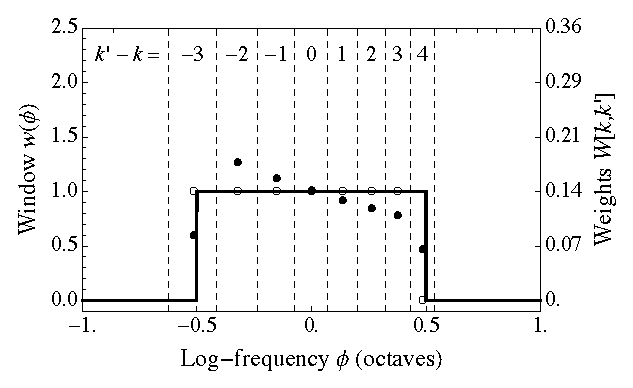
\includegraphics[width=0.6\columnwidth]{a3_smoothing_weights/figures/RectangularWeightsExample.eps}
    \caption[Calculated smoothing weights for a rectangular window function.]{
    Calculated weighting function $W[k,k']$ for methods 1 (symmetric weights -- empty circles) and 3 (log-compensated weights -- filled circles) for a rectangular window function $w(\phi)$ (solid curve).
In this example, $k = 10$ and $\Delta = 1$~octave.
Dashed vertical lines (and ticks on the top axis) indicate the limits of integration, $\Phi[10, k' \pm 0.5]$, given by \eqnref{eq:A3_Smoothing_Weights:WeightsIntegralLimits}.}
    \label{fig:A3_Smoothing_Weights:RectangularWeightsExample}
\end{figure}

The calculated non-zero weights are shown as filled circles in \figref{fig:A3_Smoothing_Weights:RectangularWeightsExample} along with the window function, both as functions of $\phi$.
From this plot, we observe two features of the weight sequence.
First, the end points take into account the extent to which the window function occupies the corresponding frequency interval, whereas simply evaluating the window function at each $k'$ would only ever give either 0 or $1/\Delta$.
Second, the intermediate points exhibit a frequency-dependent trend similar to that of a pink-noise power spectrum.
Indeed, this sequence is derived to assign equal weight per unit log-frequency (e.g., octave), so although the width of each frequency interval is constant, the ratio between the upper and lower edges of the interval decreases with increasing frequency, so the weight must also decrease.

For comparison, the weights for method 1 are also shown in \figref{fig:A3_Smoothing_Weights:RectangularWeightsExample} as empty circles that remain constant ($W[k,k'] = 1/7$) for $| k - k' | \leq m[k] = 3$ and zero otherwise.
%\end{example*}

\section{Analysis}\label{sec:A3_Smoothing_Weights:Analysis}
To examine how each smoothing method affects log-frequency symmetry, we apply each method to the magnitude response of an analog band-pass filter whose frequency response is given by
\begin{equation}
H(i \omega) = \frac{\frac{i\omega}{\omega_0}/Q}{1 + \frac{i\omega}{\omega_0}/Q + (\frac{i\omega}{\omega_0})^2}.
\end{equation}
In this analysis, we choose a $1/6^{\textrm{th}}$-octave band-pass filter ($Q \approx 8.65$ from \eqnref{eq:A3_Smoothing_Weights:QFactor}) with a center frequency of $f_0 = \omega_0/(2\pi) = 5000$~Hz, and sample the frequency response above at $N = 4096$ points, with a frequency resolution of $\approx24$~Hz (i.e., $F_s = 100,000$~samples/s).
The raw spectrum is then given by $X[k] = \left| H(2 \pi i k F_s / N) \right|^2$.

To quantify any skewing of log-frequency symmetry, we compare the center frequency, $f_0$, of the band-pass filter to the ``center of mass,'' $f_c$, of each smoothed spectrum.%
\footnote{There is a subtle but important distinction between the center of mass of a magnitude response (as defined here) and that of the power spectrum of a signal (also known as the ``spectral centroid'').
For a magnitude response, we can arbitrarily choose frequencies at which to sample the response, although doing so may change the result.
A signal's power spectrum, however, cannot be resampled arbitrarily, as its data points represent power per unit frequency, and therefore its center of mass is unambiguously defined.} We define $f_c$ in coordinates of log-frequency such that, for our chosen raw spectrum (which is symmetric in log-frequency), the result is equal to $f_0$.
This center of mass is given by
\begin{equation}
f_c = \exp \left( {\frac{\displaystyle \sum_{\ell = \ell_0 - \lceil 2/\beta \rceil}^{\ell_0 + \lceil 2/\beta \rceil} \log \left( \frac{\kappa[\ell] F_s}{N} \right) \hat{X_\textrm{s}} [\ell]}{\displaystyle \sum_{\ell = \ell_0 - \lceil 2/\beta \rceil}^{\ell_0 + \lceil 2/\beta \rceil} \hat{X_\textrm{s}} [\ell]}} \right),
\end{equation}
where $\hat{X_\textrm{s}}$ is the smoothed spectrum interpolated to a log-frequency scale, obtained using~\eqnref{eq:A3_Smoothing_Weights:LogInterpolate} with $X_\textrm{s}$ in place of $X$, and $\ell_0$ is the log-frequency index corresponding to the center frequency $f_0$ of the band-pass filter, given by
\begin{equation*}
\ell_0 = \textrm{Round} \left[ \left( \frac{N}{2} - 1 \right) \log_{N/2} \left( \frac{N f_0}{F_s} \right) \right].
\end{equation*}
The limits of the summation, $\ell_0 \pm \lceil 2/\beta \rceil$, indicate averaging over two octaves above and two below $f_0$.
The error in the center of mass is then given in percent by
\begin{equation}
\epsilon = 100 \times \frac{f_c - f_0}{f_0}.
\end{equation}

%%%% RESULTS %%%%
\subsection{Results} \label{sec:A3_Smoothing_Weights:Results}
The differences between the three smoothing methods can be seen qualitatively in \figref{fig:A3_Smoothing_Weights:SmoothedBPFExample}, which shows the smoothed spectra produced by each of these methods using rectangular windows and 1-octave smoothing.
We see from this plot that not only is method 1 unable to preserve the log-frequency symmetry observed in the raw spectrum, but also the smoothed spectrum for method 1 appears shifted to the right (i.e., blue-shifted) relative to those of methods 2 and 3 and to the original spectrum.

\begin{figure}[t]
    \centering
    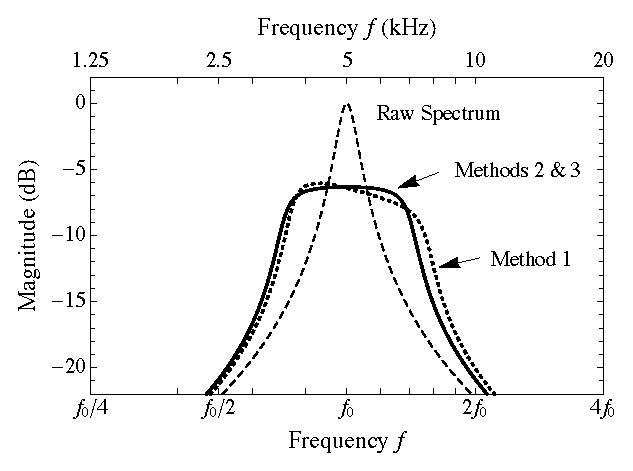
\includegraphics[width=0.6\columnwidth]{a3_smoothing_weights/figures/SmoothedBPFExample.eps}
    \caption[Original and smoothed magnitude responses of a band-pass filter.]{
    Original and 1-octave-smoothed spectra for the magnitude response of an analog band-pass filter.
Method 1 refers to the symmetric weights method; 2 to interpolation to a log-frequency scale; and 3 to log-compensated weights.
The smoothed spectra produced by methods 2 and 3 are nearly identical, so both are represented by the black curve.
The bottom axis shows frequency relative to the center frequency, $f_0$, of the band-pass filter, while the top axis shows frequency in kHz for $f_0 = 5$~kHz.}
    \label{fig:A3_Smoothing_Weights:SmoothedBPFExample}
\end{figure}

The errors in the center of mass are plotted in \figref{fig:A3_Smoothing_Weights:CenterOfMassAnalysis} for each smoothing method and for a range of smoothing bandwidths.
We see from this plot that the center of mass of the smoothed spectrum generated by method 1 increases in frequency as smoothing bandwidth increases.
For small smoothing bandwidths ($\Delta < 1/3$~octave), this error is quite small ($< 1\%$), but becomes large ($\sim 10\%$) for large smoothing bandwidths.

\begin{figure}[t]
    \centering
    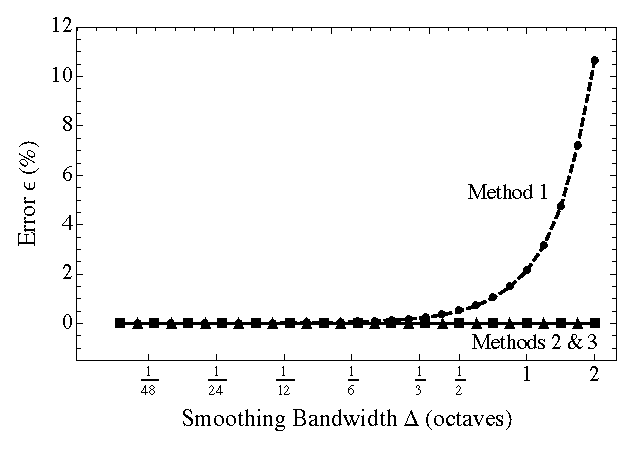
\includegraphics[width=0.6\columnwidth]{a3_smoothing_weights/figures/CenterOfMassAnalysis.eps}
    \caption[Error in the center of mass for different smoothing bandwidths.]{
    Error, $\epsilon$, in the center of mass for different smoothing bandwidths, $\Delta$.
Method 1 refers to the symmetric weights method (denoted by filled circles); 2 to interpolation to a log-frequency scale (triangles); and 3 to log-compensated weights (squares).
Plot markers for methods 2 and 3 are alternated for legibility.}
    \label{fig:A3_Smoothing_Weights:CenterOfMassAnalysis}
\end{figure}

Contrary to the center of mass, the maximum of the smoothed spectrum for method 1 appears shifted to the \textit{left} relative to that of the original spectrum (see \figref{fig:A3_Smoothing_Weights:SmoothedBPFExample}).
To further explore this phenomenon, we apply methods 1 and 3 to smooth a unit impulse located at $f_0$, as shown in \figref{fig:A3_Smoothing_Weights:SmoothingImpulseResponse}.
From this plot we see that the maximum of the smoothed spectrum for method 1 occurs at a significantly lower frequency than $f_0$, although the precise location of the maximum will depend on the raw spectrum (e.g., the width of the raw peak), the smoothing window, and the smoothing bandwidth.

\begin{figure}[t]
    \centering
    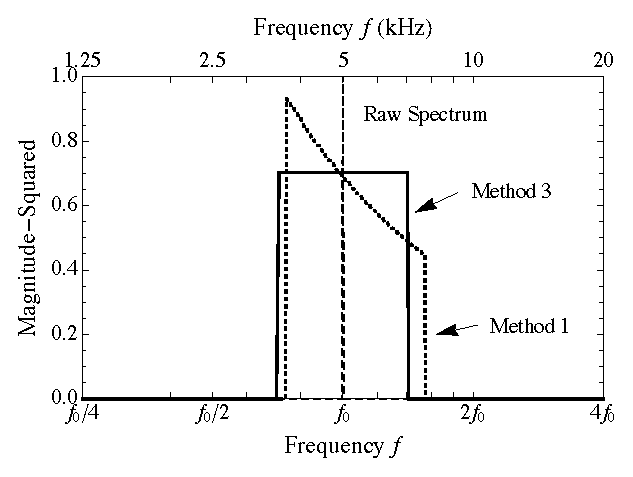
\includegraphics[width=0.6\columnwidth]{a3_smoothing_weights/figures/SmoothingImpulseResponse.eps}
    \caption[Original and smoothed spectra for a unit impulse.]{
    Original and 1-octave-smoothed spectra for a unit impulse located at $f_0$, computed for methods 1 (symmetric weights) and 3 (log-compensated weights).
The smoothed spectra are multiplied by a factor of 100 for legibility.
The bottom axis shows frequency relative to $f_0$, while the top axis shows frequency in kHz for $f_0 = 5$~kHz.}
    \label{fig:A3_Smoothing_Weights:SmoothingImpulseResponse}
\end{figure}

The reason for this shift can be understood in terms of the contribution of the raw spectrum's maximum to each smoothed value.
From \eqnreftwo{eq:A3_Smoothing_Weights:HatzHalfWidth}{eq:A3_Smoothing_Weights:HatzWeights}, as frequency $k$ increases, the width of the smoothing window increases and, due to the normalization of the weights, its amplitude decreases.
Consequently, the contribution of the raw spectrum's maximum to the smoothed value decreases as frequency increases, yielding, in this case, a steadily decreasing smoothed spectrum.

Method 3, on the other hand, creates a uniform spectrum that is symmetric about $f_0$, but has no single maximum.
However, it can be verified that for other smoothing windows (e.g., Hanning), the peak appears at $f_0$.

\section{Conclusions}\label{sec:A3_Smoothing_Weights:Conclusions}
In this work we explored the ability (or lack thereof) of fractional-octave smoothing methods to preserve the log-frequency symmetry of frequency spectra.
Specifically, we examined two existing methods of smoothing, the first of which uses a symmetric (on a linear frequency scale) window of the correct bandwidth, but whose cutoff frequencies are not equidistant from the center frequency when viewed on a log-frequency scale, and therefore do not correspond to the \textit{correct} fractional-octave band.
The second method requires that the raw spectrum first be interpolated to a log-frequency scale, a process that necessarily introduces errors, but simplifies the fractional-octave smoothing procedure to a moving-average operation with a symmetric window that corresponds well with the correct fractional-octave band.
We proposed a third smoothing method that is able to accurately replicate the smoothed spectrum of the second method but without the need for interpolation.
This method is fully compatible with other FFT-based smoothing techniques such as complex smoothing (see \citet{HatziantoniouMourjopoulos2000}) and can be employed with any smoothing window (e.g., Hanning window, band-pass filter, etc.), provided the window can be specified as an integrable function of log-frequency.

We performed a numerical analysis of the ``center of mass'' of the smoothed spectra produced by each method given the magnitude response of an analog band-pass filter (which is symmetric on a log-frequency scale) as the raw spectrum.
This analysis revealed that only the first method is unable to preserve the log-symmetry of the raw spectrum, as it shifts the center of mass upwards in frequency, resulting in a ``blue-shifted'' smoothed spectrum.
It is worth noting that this error is quite small for small smoothing bandwidths (e.g., the center of mass shifts by $< 1 \%$ of the center frequency for $1/3$-octave smoothing) and therefore may be tolerable in some applications.
We also smoothed a unit impulse with the first and third methods to explore how the maximum may shift after smoothing.
Results showed that only the first method shifts the maximum downwards in frequency, although we expect this phenomenon to be less significant for smaller smoothing bandwidths.

Regarding the computational cost of the proposed method, it is relevant to note that, for many smoothing windows, the definite integral of the window (see \eqnref{eq:A3_Smoothing_Weights:WeightsIntegral}) can be evaluated analytically, making the calculation of each weight sequence computationally inexpensive.
Furthermore, for all smoothing windows, the weighting function can be precomputed and stored in a matrix, recasting the smoothing operation as a matrix multiplication whose computational expense would be invariant with smoothing method, window, and bandwidth.

Future work should include an exploration of the equivalent time-domain implementation of the proposed method, wherein smoothing is expressed as multiplication of the input impulse response with frequency-dependent windows \citep{HatziantoniouMourjopoulos2000} and an investigation into the perceptual differences, if any, between the first and third methods for various smoothing bandwidths and in various applications (e.g., digital room correction, headphone equalization, etc.).

\section*{Acknowledgements}
This work was originally published by \citet{Tylka2017} in \textit{The Journal of the Audio Engineering Society}.
The present author wishes to thank R.~Sridhar for fruitful discussions during this work and the anonymous reviewers for their feedback.